\documentclass[aspectratio=169]{beamer}
\usepackage[utf8]{inputenc}
\usepackage{bbding}
\usepackage[weather]{ifsym}
\usepackage{color}
\usepackage{hyperref}
\usepackage{pgfpages}
\usepackage{transparent}
\usepackage{lmodern}
\usepackage{enumitem}


\title{myHelsana Deployment Pipeline}

\subtitle{Fast Flow}


\author{Bastian Bukatz}
\institute{Innovation Process Technology}
\date{\today}

\usepackage{helvet}
\renewcommand{\familydefault}{\sfdefault}


\definecolor{ice-blue}{RGB}{162,210,223}
\definecolor{ipt-blue}{cmyk}{1,0.45,0.18,0.07}
\definecolor{ipt-red}{cmyk}{0,1,0.53,0}
\setbeamercolor{title}{fg=ipt-blue}
\setbeamercolor{frametitle}{fg=ipt-blue}
\setbeamercolor{normal text}{fg=black}
\setbeamercolor{alerted text}{fg=ipt-red}
\setbeamercolor{section in toc}{fg=ipt-blue}
\setbeamercolor{item}{fg=ipt-blue}


\usepackage{hyperref}
\hypersetup{colorlinks=true,linkcolor=ipt-blue,urlcolor=ipt-blue}

\makeatletter
\setbeamertemplate{frametitle}{
    \ifbeamercolorempty[bg]{frametitle}{}{\nointerlineskip}%
    \@tempdima=\textwidth%
    \advance\@tempdima by\beamer@leftmargin%
    \advance\@tempdima by\beamer@rightmargin%
    \hspace*{0.3cm} %%%%%%%%%%%%% For example insert shift to right
    \begin{beamercolorbox}[sep=0.3cm,wd=\the\@tempdima]{frametitle}
        \usebeamerfont{frametitle}%
        \vbox{}\vskip-1ex%
        \if@tempswa\else\csname beamer@ftecenter\endcsname\fi%
        \strut\insertframetitle\strut\par%
        {%
            \ifx\insertframesubtitle\@empty%
            \else%
            {\usebeamerfont{framesubtitle}\usebeamercolor[fg]{framesubtitle}\insertframesubtitle\strut\par}%
            \fi
        }%
        \vskip-1ex%
        \if@tempswa\else\vskip-.3cm\fi% set inside beamercolorbox... evil here...
    \end{beamercolorbox}%
}
\makeatother


\begin{document}

\usebackgroundtemplate{
\includegraphics[width=\paperwidth]{pictures/ipt_titelpage2.jpg}}
\begin{frame}
\titlepage
\end{frame}


\usebackgroundtemplate{
\includegraphics[width=\paperwidth]{pictures/ipt_standardpage.jpg}}

\begin{frame}
\frametitle{Table of Contents}
\tableofcontents
\end{frame}


\section{Einleitung}
\subsection{Management Summary}
\begin{frame}
\frametitle{\subsecname}\framesubtitle{\secname}
Im folgenden werden einige Voraussetzungen erklärt.
\end{frame}

\begin{frame}

\subsection{Was ist eine Deployment Pipeline}
\frametitle{\subsecname}\framesubtitle{\secname}
deployment pipeline's job is to detect any changes that will lead to problems in production. These can include performance, security, or usability issues. A deployment pipeline should enable collaboration between the various groups involved in delivering software and provide everyone visibility about the flow of changes in the system, together with a thorough audit trail.
\begin{itemize}[label={$\bullet$}]
\item Fail Early: Alle Probleme die in Produktion auftreten können so früh es geht festestellen.
\end{itemize}
\end{frame}


\subsection{Vorgehen}
\begin{frame}
\frametitle{\secname}\framesubtitle{\subsecname}
A good way to introduce continuous delivery is to model your current delivery process as a deployment pipeline, then examine this for bottlenecks, opportunities for automation, and collaboration points.
\begin{itemize}[label={$\bullet$}]
\item Model your value stream and create a walking skeleton.
\item Automate the build and deployment process.
\item Automate unit tests and code analysis.
\item Automate acceptance tests.
\item Automate releases.
\end{itemize}

\href{http://www.informit.com/articles/article.aspx?p=1621865&seqNum=8}{Vorgehen nach Martin Fowler}
\end{frame}



\subsection{Umdenken im Testing}
\begin{frame}
\frametitle{\subsecname}\framesubtitle{\secname}
\centering
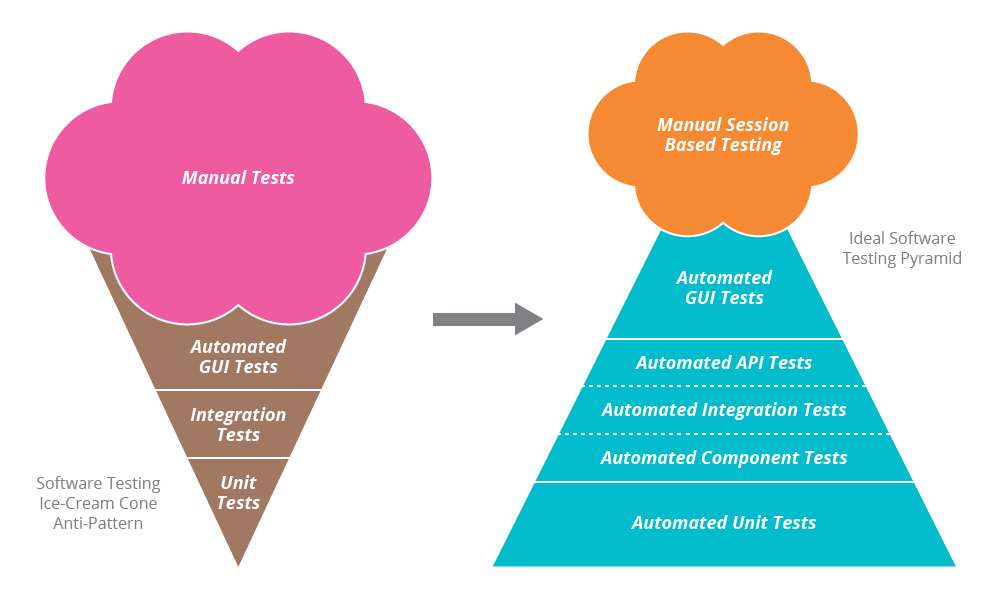
\includegraphics[width=0.7\textwidth]{pictures/TestPyramid.png}
\vfill
\begin{figure}[!b]
  Burnes, B. (2004). \href{http://doi.org/10.1111/j.1467-6486.2004.00463.x}{Kurt Lewin and the planned approach to change: A re-appraisal}. Journal of Management Studies.
\end{figure}
\end{frame}

\end{document}
